% Full instructions available at:
% https://github.com/elauksap/focus-beamertheme

\documentclass[9pt]{beamer}
\usetheme{focus}

%%%%%%%%%%%%%%%%%%%%%%%%%%%%%%%%%%%%%%%%%%%%%%%%%%%%%%%%%%%%%%%%%%%%%
% Typography, change document font
\usepackage[tt=false, type1=true]{libertine}
\usepackage[varqu]{zi4}
\usepackage[libertine]{newtxmath}
\usepackage[T1]{fontenc}

\usepackage[protrusion=true,expansion=true]{microtype}

% Disable paragraph indentation, and increase gap
\usepackage{parskip}

%Matrix
\usepackage{tabstackengine}
\setstackEOL{;}% row separator
\setstackTAB{,}% column separator
\setstacktabbedgap{1ex}% inter-column gap 
\setstackgap{L}{1.0\normalbaselineskip}% inter-row baselineskip
\let\mat\bracketMatrixstack

\newcommand{\pth}{Figure/}
\newcommand{\ve}[1]{\mathbf{#1}}

% Copyright (C) 2018-2019 Pasquale Claudio Africa and the LaTeX community.
% A full list of contributors can be found at
%
%     https://github.com/elauksap/focus-beamertheme
% 
% This file is part of beamerthemefocus.
% 
% beamerthemefocus is free software: you can redistribute it and/or modify
% it under the terms of the GNU General Public License as published by
% the Free Software Foundation, either version 3 of the License, or
% (at your option) any later version.
% 
% beamerthemefocus is distributed in the hope that it will be useful,
% but WITHOUT ANY WARRANTY; without even the implied warranty of
% MERCHANTABILITY or FITNESS FOR A PARTICULAR PURPOSE. See the
% GNU General Public License for more details.
% 
% You should have received a copy of the GNU General Public License
% along with beamerthemefocus. If not, see <http://www.gnu.org/licenses/>.

\mode<presentation>


% DEFINE COLORS. ---------------------------------------------------------------
\definecolor{main}{RGB}{134, 161, 174}
\definecolor{main2}{RGB}{104, 131, 144}
\definecolor{textc}{RGB}{20, 20, 20}
\definecolor{background}{RGB}{255, 255, 255}

\definecolor{alert}{RGB}{180, 0, 0}
\definecolor{example}{RGB}{0, 110, 0}


% SET COLORS. ------------------------------------------------------------------
\setbeamercolor{normal text}{fg=textc, bg=background}
\setbeamercolor{alerted text}{fg=textc}
\setbeamercolor{example text}{fg=textc}

\setbeamercolor{titlelike}{fg=background, bg=main}
\setbeamercolor{frametitle}{parent={titlelike}}

\setbeamercolor{footline}{fg=background, bg=main2}

\setbeamercolor{block title}{bg=main!80!background, fg=background}
\setbeamercolor{block body}{bg=main!10!background, fg=textc}

\setbeamercolor{block title alerted}{bg=alert, fg=background}
\setbeamercolor{block body alerted}{bg=alert!10!background, fg=textc}

\setbeamercolor{block title example}{bg=example, fg=background}
\setbeamercolor{block body example}{bg=example!10!background, fg=textc}

\setbeamercolor{itemize item}{fg=textc}
\setbeamercolor{itemize subitem}{fg=textc}

\setbeamercolor{enumerate item}{fg=textc!70!black}
\setbeamercolor{enumerate subitem}{fg=textc!70!black}

\setbeamercolor{description item}{fg=textc!70!black}
\setbeamercolor{description subitem}{fg=textc!70!black}

\setbeamercolor{caption name}{fg=textc}

\setbeamercolor{section in toc}{fg=textc}
\setbeamercolor{subsection in toc}{fg=textc}
\setbeamercolor{section number projected}{bg=textc}
\setbeamercolor{subsection number projected}{bg=textc}

\setbeamercolor{bibliography item}{fg=main}
\setbeamercolor{bibliography entry author}{fg=main!70!black}
\setbeamercolor{bibliography entry title}{fg=main}
\setbeamercolor{bibliography entry location}{fg=main}
\setbeamercolor{bibliography entry note}{fg=main}

\mode<all>


\begin{document}
	\tableofcontents	
\section{Linearity and non-linearity : \today}
	\begin{frame}
		\begin{itemize}
			\item Suppose there is a function or mapping that does this $f : x \rightarrow y$. Function f takes x and gives y
			
			\item The function is linear if $f(x) = f(x_1) + f(x_2)$. where $x = x_1 + x_2$
			
			\item Suppose we know $f()$ and $y$ but not $x$. Because the function is linear, we can construct solutions $x$ that may be a combination of different solutions $x_i$. The idea is that $f$ should not depend on $x$. It can have other parameters, but not the values of the solution itself. In that case, we would have to find the solution $x$ and also the mapping $f$
			
		\end{itemize}
	
		\begin{block}{Example}
			Take function or map () 
		\end{block}
	\end{frame}




\section{Structural non-linearity introduction}
	\begin{frame}
		\begin{itemize}
			\item What does non-linearity mean ?
			\item What makes a structure non-linear ?
			\item How do you model non-linearity and solve it?
		\end{itemize}
	\end{frame}
	
	\begin{frame}{Structural non-linearity }
		\begin{itemize}
		\item There are different types of non-linearity in a structure 
		\begin{itemize}
			\item Geometrical - $\ve{K(x)x = F }$ where here $\ve{K}$ depends on $\ve{x}$ because $\ve{K}$ changes as you chagne x due to the change in geometry and the large deformation.  
			\item Material - $\ve{K(x)x = F }$ because $\ve{K}$ changes due to the changes in the material property. For eg Youngs modulus may be a function of x. 
		\end{itemize}
		\item $\ve{K}$ is now a function of (x), it means that it can't be solved by using a linear method (Inverting a matrix). 
		\item But the system of equations now has to be linearised about a point. 
		We keep the system of equations as an equality equation $\ve{K(x)x - F} = 0$ . 
		\item We linearise and try to solve the root. At every point we construct the tangent and find a solution, but when we construct the solution at that point, we find the residual and we then use to iterate until convergence. 	
		\end{itemize}
	\end{frame}
		
	\begin{frame}{Problem \#1}
		\begin{figure}
			\centering
			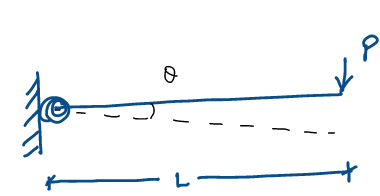
\includegraphics[width=0.7\linewidth]{Figure/fig1}
			\caption{}
			\label{fig:fig1}
		\end{figure}
		Taking a weightless rigid bar with a torsional spring that resists any moment and a load P at the end. Since the bar is rigid so vertical equilibrium is satisfied at the support without any deformation. However, it can rigidly rotate through the spring.
	\end{frame}
	
	\begin{frame}
		 The moment generated at the end support is	 
		\begin{equation}
			PL cos \theta = M
		\end{equation}
		Taking the equilibrium equation with the spring as $ M = K \theta$ we get
		\begin{align*}
		PL cos \theta = K \theta \\
		\frac{PL}{K} = \frac{\theta}{cos \theta}
		\end{align*}
		\begin{itemize}
			\item If we take $\theta \rightarrow 0$ then $cos \theta \rightarrow 1$
			\item So $P = \dfrac{K}{L}\theta$ which is linear wrt $\theta$
		\end{itemize}
	\end{frame}

	\begin{frame}
		\begin{itemize}
			\item Linearity : $\dfrac{PL}{K} = {\theta}$
			\item Geometric nonlinearity only : $\dfrac{PL}{K} = \dfrac{\theta}{cos \theta}$
			\item Material nonlinearity only : $\dfrac{PL}{K(\theta)} = {\theta}$ \footnote{We can say the spring stiffness as a material parameter K that also depends on $\theta$ introducing the material nonlinearity. For eg, we can model $K(\theta) = K_o(1-c\theta)$}
			\item Geometric + Material nonlinearity : $\dfrac{PL}{K(\theta)} = \dfrac{\theta}{cos \theta}$
		\end{itemize}
	\end{frame}

	\begin{frame}{Problem \#2}
		\begin{figure}
			\centering
			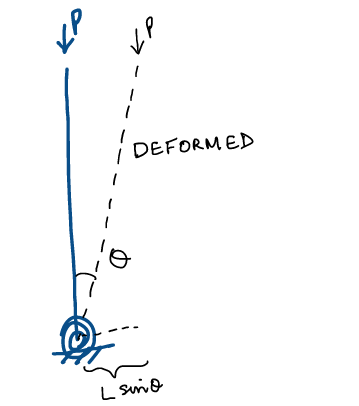
\includegraphics[width=0.4\linewidth]{Figure/fig2}
			\caption{}
			\label{fig:fig1}
		\end{figure}
		Same problem but now the rigid bar is vertical. This is a very common problem for nonlinearity (I think the previos one is better tho!). Nicely represents buckling of columns
	\end{frame}

	\begin{frame}
		Same equilibrium equation but now the lever arm is different (Because the load along the bar)
		\begin{equation}
		PL sin \theta = M
		\end{equation}
		Taking the equilibrium equation with the spring as $ M = K \theta$ we get
		\begin{align*}
		PL sin \theta = K \theta \\
		\frac{PL}{K} = \frac{\theta}{sin \theta}
		\end{align*}
		\begin{itemize}
			\item If we take $\theta \rightarrow 0$ then $sin \theta \rightarrow 0$ so $M = 0$ (This is one possible equilibrium)
			\item	$\frac{PL}{K} = \frac{\theta}{sin \theta}$ : This is the other
			\item The load $\frac{PL}{K}$ where these two equilibrium equations are possible for the same structure is called the bifurcation point. 
			\item You can imagine that when the load is smaller, it will not buckle and only deform axially so only one equilibrium position ($\theta =0$) is possible. When $\frac{PL}{K}>1$ then the other equilibrium comes to play.
		\end{itemize}
	\end{frame}

	\begin{frame}
		Therefore two solutions  are there :
		\begin{figure}
			\centering
			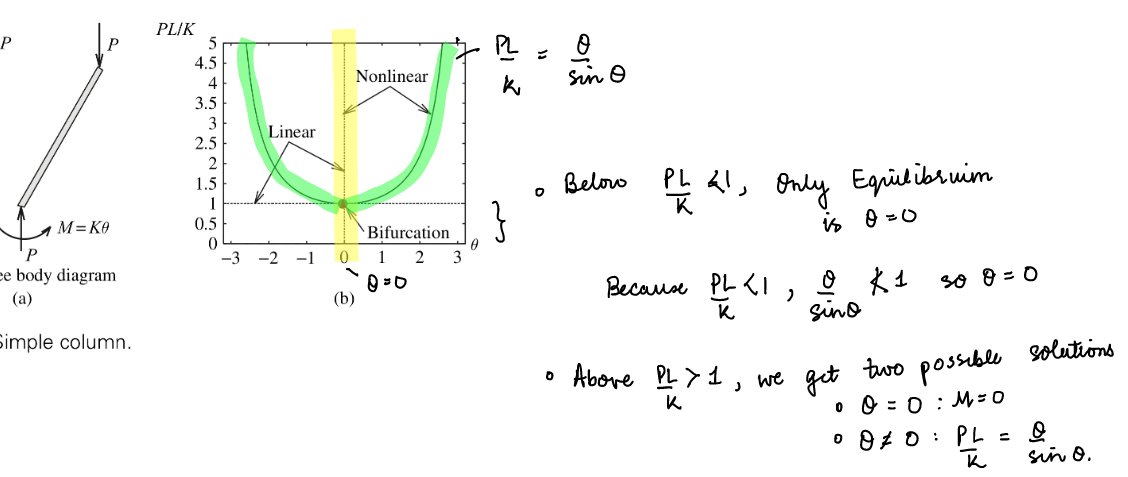
\includegraphics[width=1\linewidth]{Figure/fig3}
			\label{fig:fig3}
		\end{figure}
		\begin{itemize}
			\item If we linearise our equilibrium equation for small $\theta \rightarrow sin \theta$
			\item We get $(Pl - K)\theta = 0$ and we get our linear eigen value problem with a trivial solution of $\theta = 0$ and a nontrivial solution of $PL = K$. Again we get two equilibrium solutions. $PL = K$ being the buckling load. 
			\item So when we reach that load, it means we have reached the bifurcation point, where multiple equilibrium solutions exist and the rod may buckle dependant on imperfection, lateral load etc. 			
		\end{itemize}
	\end{frame}

\end{document}